%	\section{Experiment 0: Explicit Evaluations}
%	In order to establish a baseline gender score for morphologically marked gendered occupational and social roles in English, blah...
%	
%	\subsection{Methods} 
%	
%	100 participants were recruited through the online recruitment platform `Prolific'. All participants self-identified as L1 English speakers and as having been born and in the United States, and all lived in the United States at the time of participation. None of the participants had participated in the pilot study. Finally, all participants were paid \$2.00 for their participation in the study, and spent an average of four to five minutes on the experiment (average payout \$31.86 per hour). 
%	
%	Each participant was presented with a series of sentences of the form ``Someone is a TITLE", where the title in question was one of the 39 selected titles in one of their gendered forms. Each participant saw all 39 of the lexical items in question, and 13 of each gender form (male/female/neutral), so that no participant ever saw the same lexeme in a different format (e.g. a participant would not see both \textit{congressperson} and \textit{congresswoman}). 
%	
%	Participants were asked to judge how likely it was that the `someone' in question was a man or a woman, and indicated their responses on a seven-point Likert scale. Which binary gender the left (1) or right (7) ends of the scale represented was randomized between participants but consistent within a single subject's study. For each item, participants were also permitted to check an optional box indicating that they were not familiar with the term in question, due to the relatively low frequency of some of the critical items.  Finally, all participants completed an optional post-experiment demographic survey.
%	
%	%An example of this procedure is provided in Figure \ref{norming_sample}.
%	
%%	\begin{figure*}[hb]
	%%		\centering
	%%		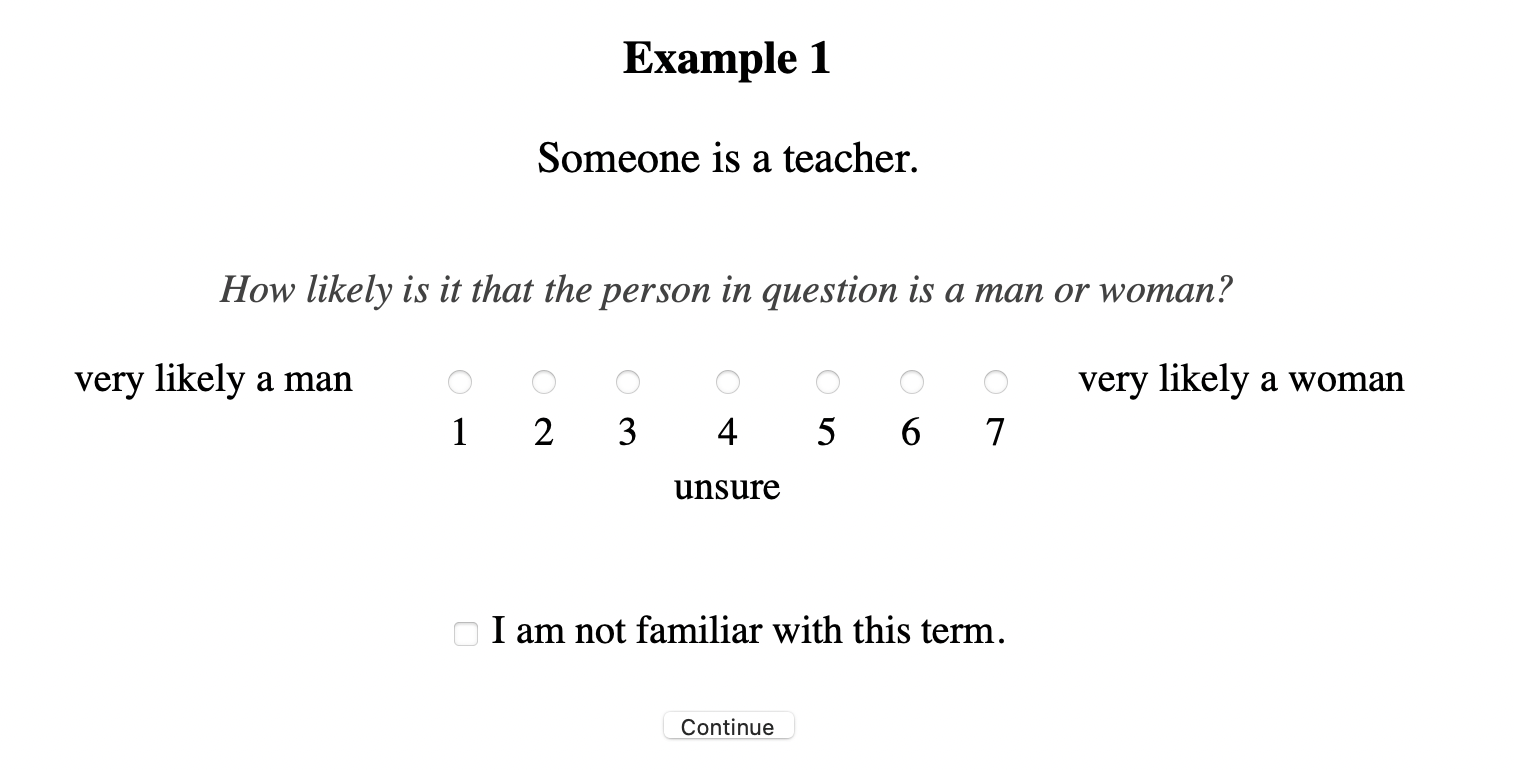
\includegraphics[scale=0.5]{norming_capture.png}
	%%		\caption{A trial of the procedure in Experiment 0, as seen by participants}
	%%		\label{norming_sample}
	%%	\end{figure*}
%	
%	
%	\subsection{Results}
%	
%	\begin{figure*}[ht]
	%		\centering
	%		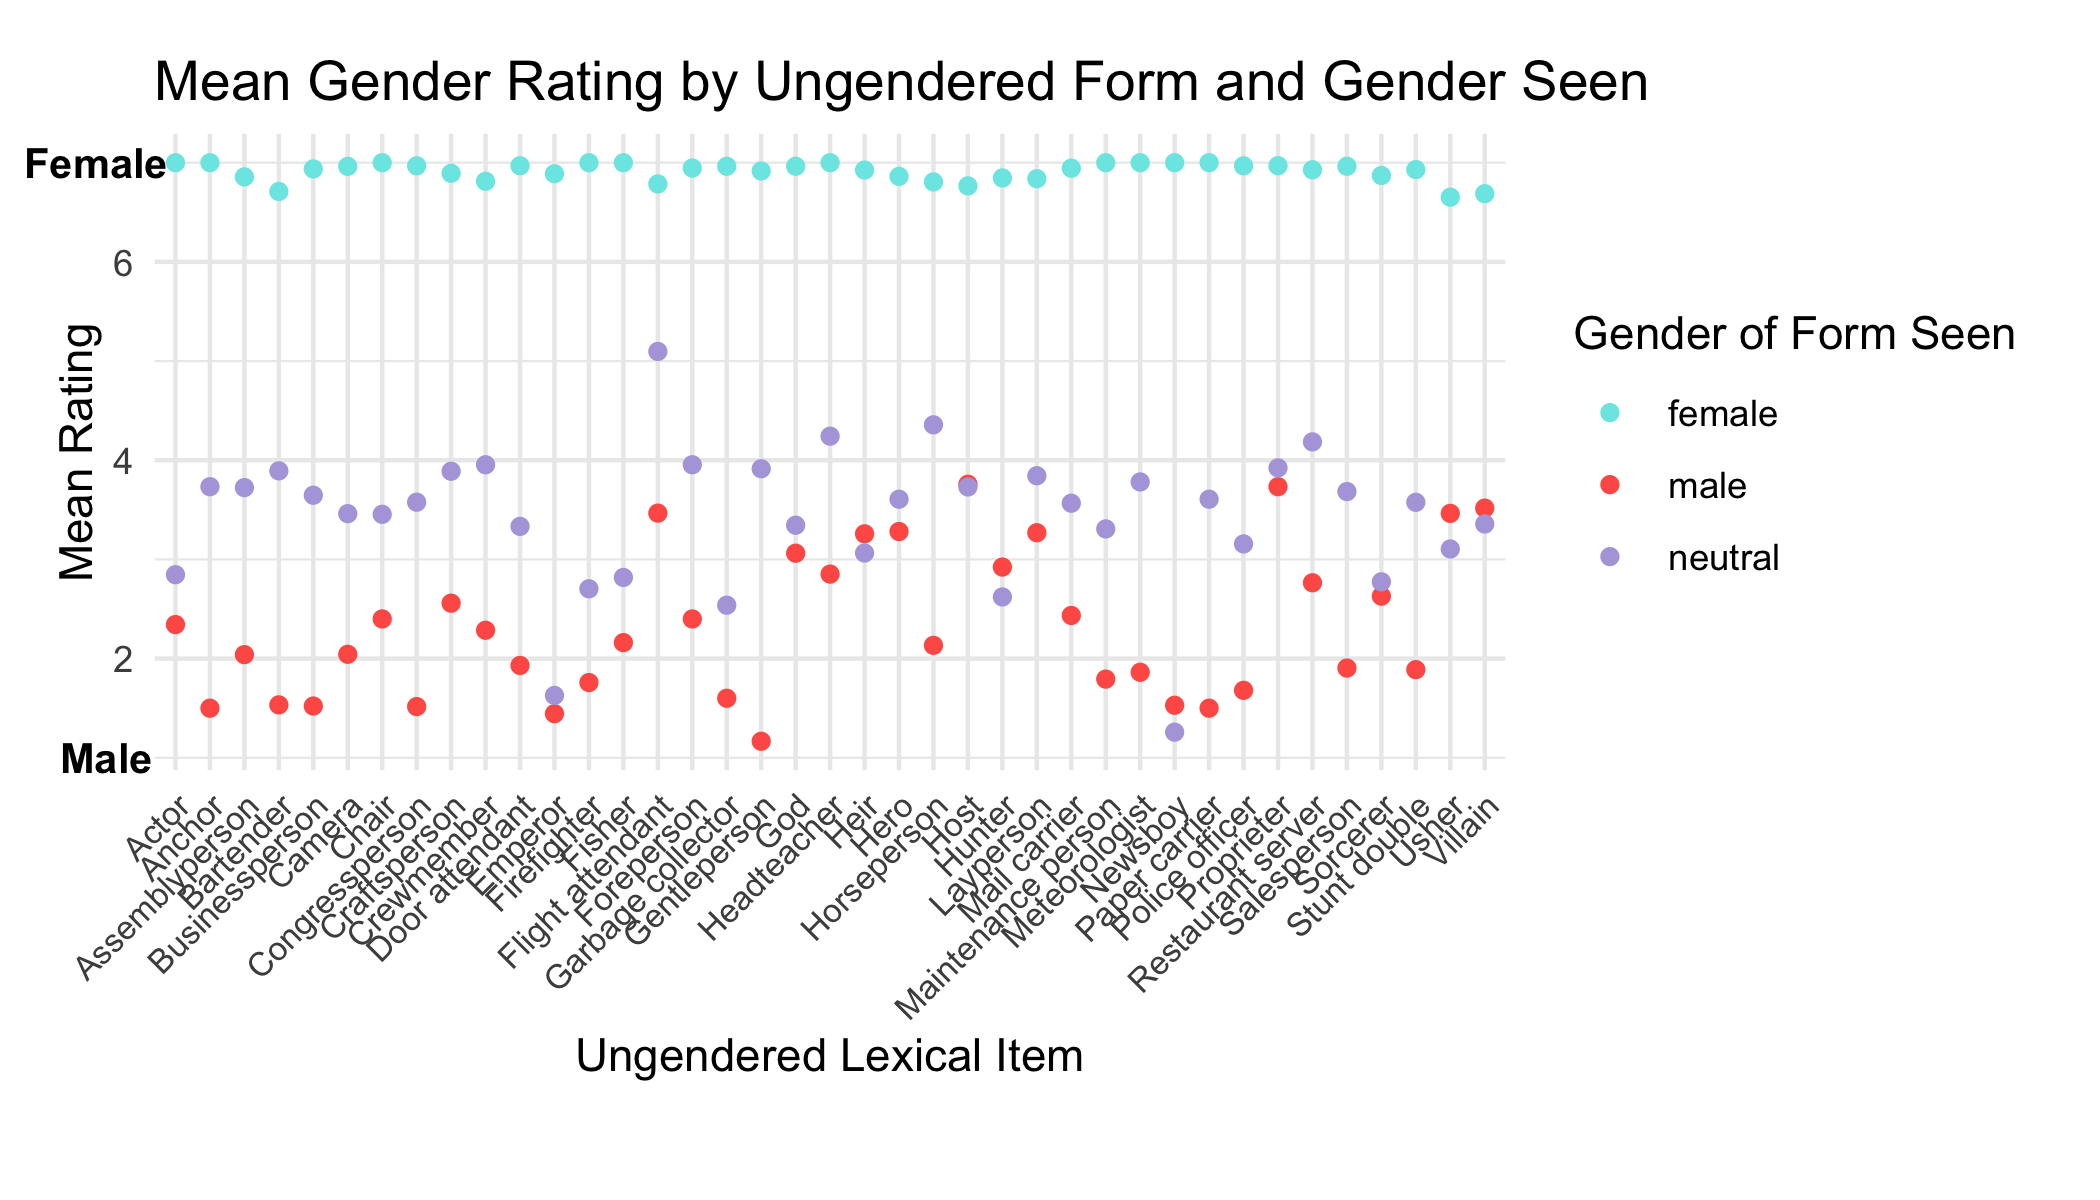
\includegraphics[scale=0.2]{norming_results_all.png}
	%		\caption{Mean gender reporting of items by lexical item and gender seen}
	%		\label{norming_results_all}
	%	\end{figure*}
\newpage
%	\section{Experiment 1: MAZE Task}
%
%	\subsection{Methods}
%	
%	\subsubsection{Participants} A total of 200 participants were collected for this task via the online recruitment platform Prolific. The task was advertised to 100 self-identifying Republicans and 100 self-identifying Democrats, in order to ensure an even distribution of political affiliations. All participants additionally self-identified as L1 English speakers and as having been born and in the United States, and all lived in the United States at the time of participation. None of the participants had participated in the pilot study or in any other study related to the present project. Finally, all participants were paid \$1.75 for their participation\footnote{With a mean completion time of 5.39 minutes, participants were paid at a rate of \$20.73/hr}. \par 
%	
%	\subsubsection{Stimuli}
%	The stimuli sentences in this experiment were of the form ``NAME is a/n TITLE from STATE. PRONOUN likes ACTIVITY"- for example, ``Brittany is a chef from Louisiana". The twenty most popular male and female names were selected from the lists of most popular names for boys and girls in 1998 according to the Social Security \citeA{socialsecurity}. Names which appeared within the top 100 entries on both lists (e.g. Taylor, Ryan) were excluded, in order to ensure that the names used in the experiment were sufficiently socially gendered. These names were randomized between participants, with no participant seeing the same name more than once. States and activities were randomized at the stimuli creation stage so that they remained constant for all participants.\par
%	The critical items in question were the forms that appeared in the TITLE location of the sentences. A total of 20 social and occupational titles which display overt morphological gender were chosen, with the majority of these showing three possible gender realizations: male, female, and neutral (e.g. \textit{congressman, congresswoman, congressperson}). The remaining items only distinguished between female and non-female forms (e.g. \textit{actress} vs. \textit{actor}). Thus, any vignette had the possibility to appear \textbf{congruent} in its gender markings (e.g. a male name with a male lexical item) or \textbf{neutral} in its congruency (e.g. a female name with a neutral lexical item)\footnote{We did not test gender-incongruent vignettes such as `David is a congresswoman', for fear that it would draw too much attention to the gendered nature of the task at hand.}. \par
%	Once the sentences were constructed, each item in the sentence was paired with a distractor item deemed to have a similar surprisal value in that same context, using the A(uto)-Maze generator developed and described in \citeA{boyce2020maze}. Where surprisal values could not be accurately obtained, for example because of low lexical frequency of the critical items, distractors were matched on orthographic length.  
%	
%	\subsubsection{Procedure}
%	The experiment consisted of an implementation of the maze task \cite{forster2009maze}, wherein participants are presented with sentences one word at a time, and each word is paired with an ungrammatical distractor. Participants are tasked with proceeding through the sentence one word at a time, selecting the grammatical continuation of the sentence by indicating a corresponding key on their keyboard, and time measures are taken of the decision time. The beginning of a sentence is always paired with an ``X-X-X", which participants are told not to select. An example of the progression of such a task is provided in Figure 1.
%	
%	\begin{figure}[ht]
	%		\centering
	%		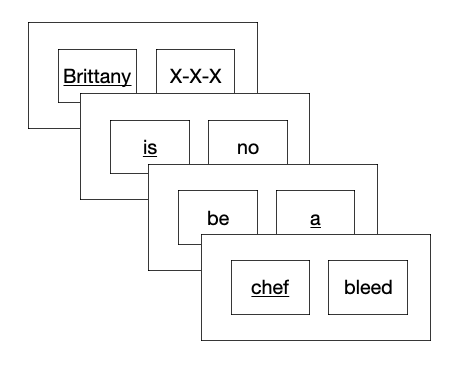
\includegraphics[scale=0.33]{maze-exe}
	%		\caption{An example of the maze task progression. Each larger frame represents a selection choice, wherein only one of the words can continue the sentence. These continuations are underlined in this example.}
	%		\label{maze-exe}
	%	\end{figure}
%	 \par 
%	If the participant successfully made it to the end of the sentence, they were asked about the state from which the character in the vignette comes. This question served both to distract participants from the question under investigation (gender) and also as an attention check. If, however, the participant failed to successfully navigate the sentence, they were prompted to continue on to the next sentence, and that item was marked as incomplete.
%
%	\subsubsection{Post-Experimental Survey}
%	In order to assess the participants' ideologies towards gender, we employ the Social Roles Questionnaire developed by \citeA{baber2006social}. This survey consists of 13 questions which are designed to elicit both implicit and explicit ideologies about gender, including the notions of gender as an immutable fact vs gender as a social construct (what Baber and Tucker term `gender transendence'), as well as about the societal roles performed by the (binary) genders (`gender linking').\par 
%	Each of the 13 questionnaire items was presented alongside a sliding scale from `strongly disagree' to `strongly agree', which corresponded to numerical values of 0 and 100, respectively. The questions related to `gender linking' were inversely coded. Participants were then assigned a gender ideology score from 0 to 100 by taking the mean of their individual responses; the closer to 0 a participant is, the more open-minded their approach to gender, and the closer to 100, the more conservative or traditional their view of gender.\par 
%	Finally, participants filled out an optional post-experimental demographic survey. This included questions about their own gender, political affiliations, and age. The full survey is available online as part of the supplementary materials.
%		
%	\subsection{Results}
%	
%	\subsubsection{Exclusions} 23 participants were excluded because they failed to meet the 80\% threshold for attention check questions. Additionally, we excluded any individual trial which deviated from the mean for that item by more than two standard deviations in order to control for the effects of outliers. This resulted in an additional 142 observations being excluded, for a total of 3271 observations left for analysis.  
%	
%	\begin{figure}[ht]
	%		\centering
	%		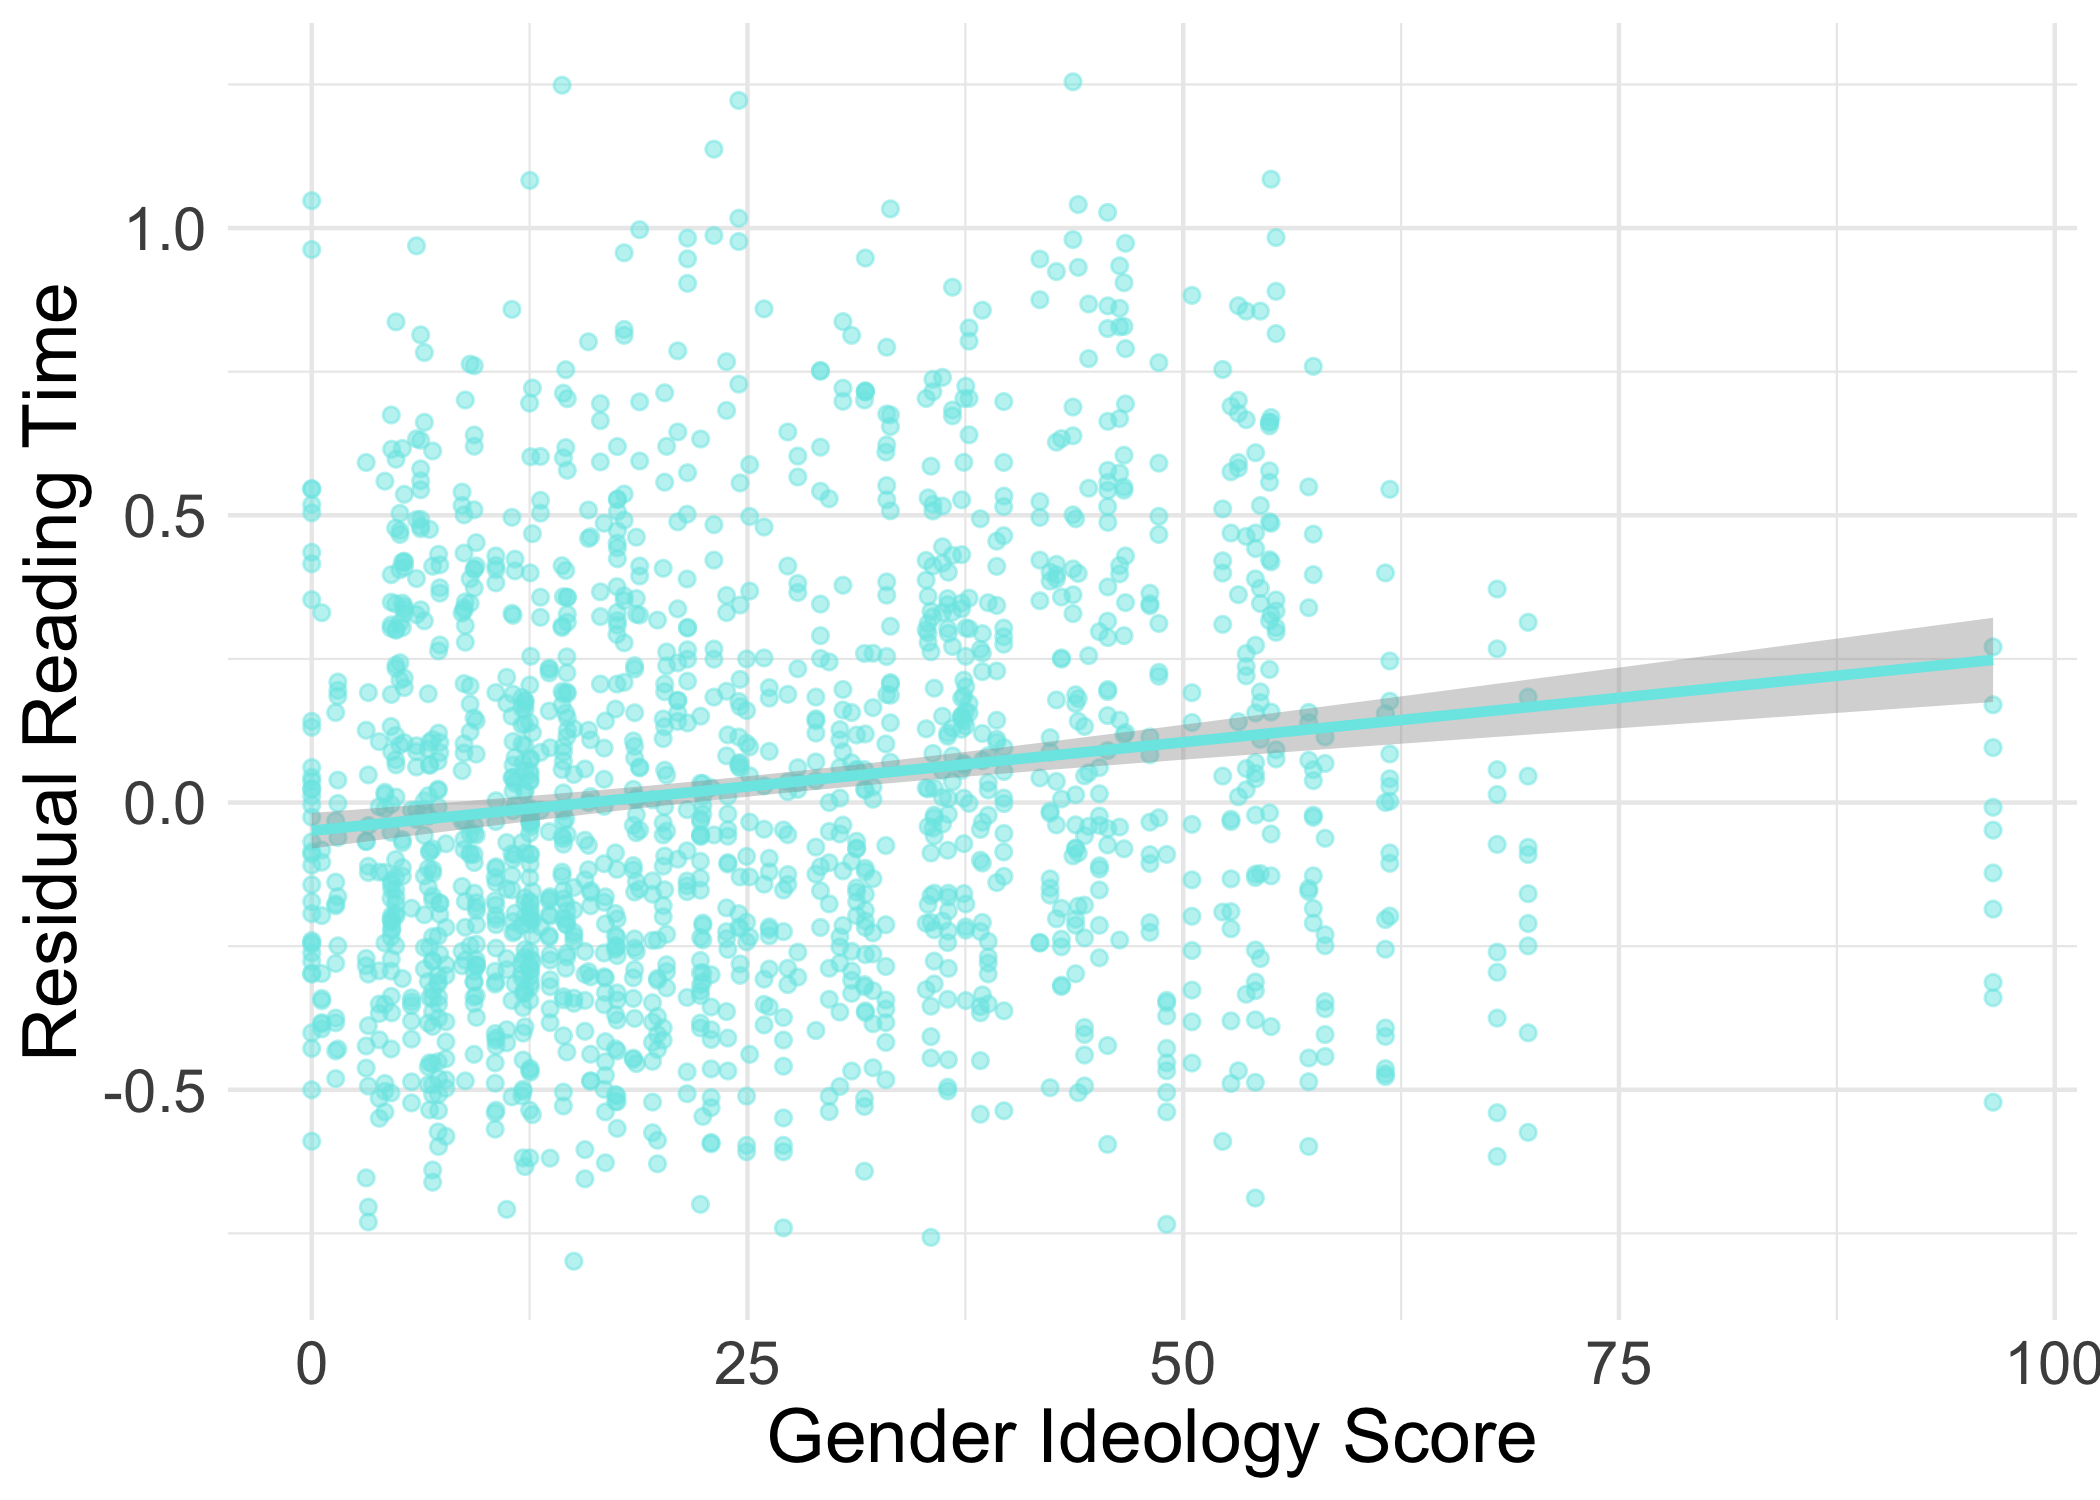
\includegraphics[scale=0.115]{maze_neutral_all.png}
	%		\caption{Average residual decision time on gender-neutral forms in Experiment 1.}
	%		\label{maze_neutral_all}
	%	\end{figure}
%	
%	\begin{figure}[ht]
	%		\centering
	%		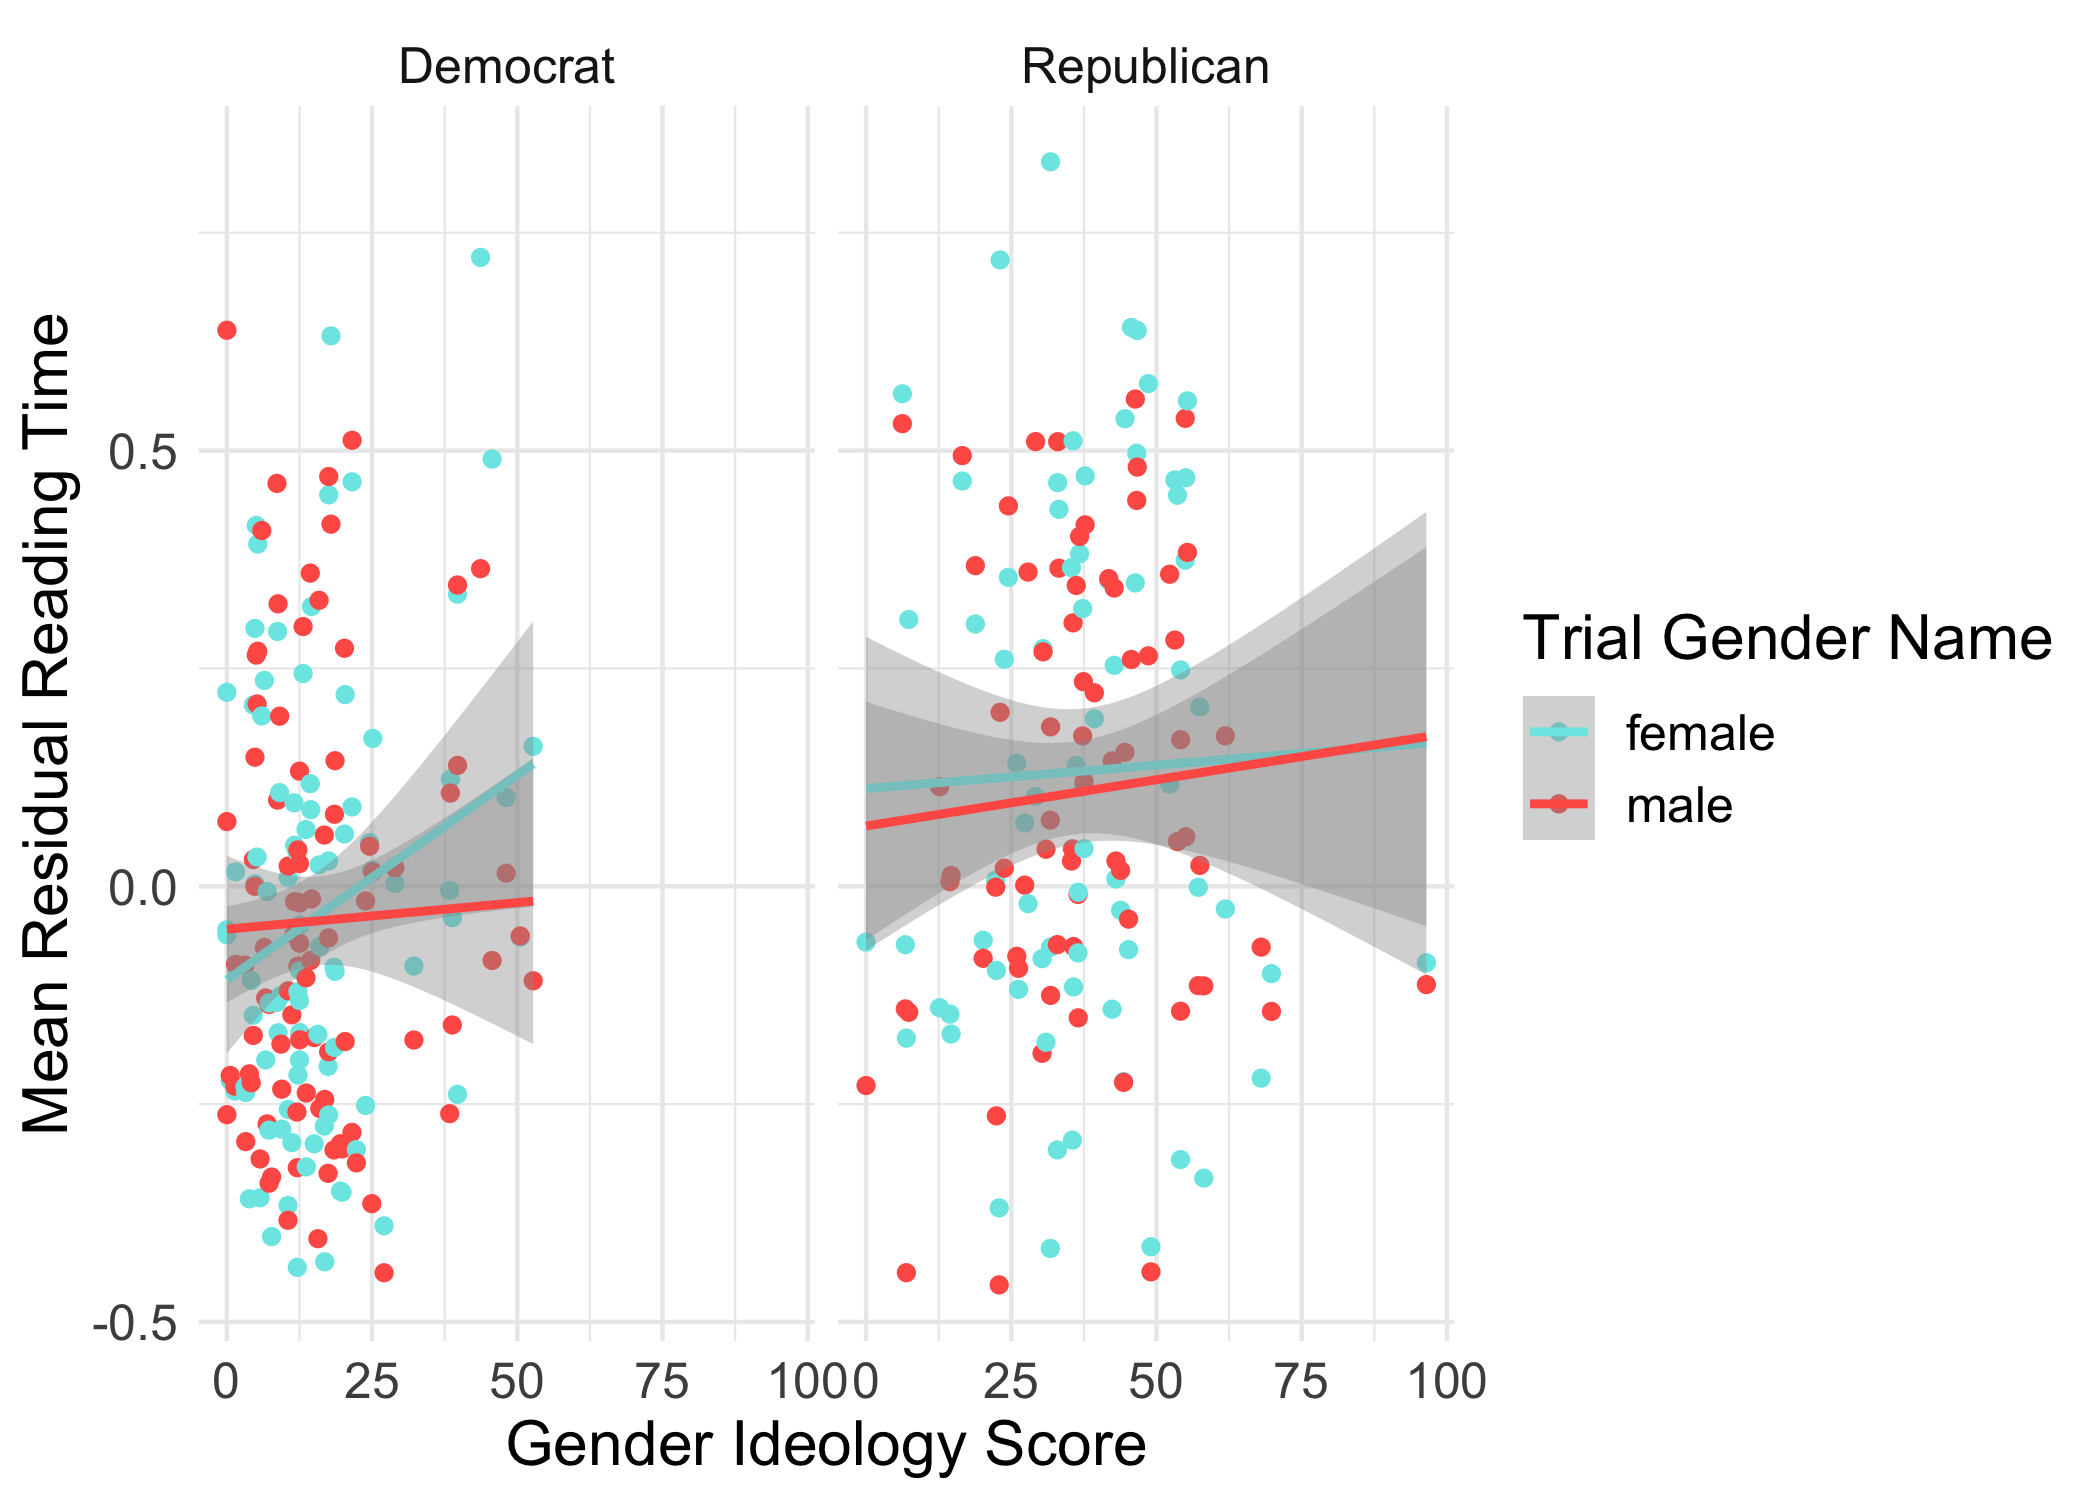
\includegraphics[scale=0.115]{maze_neutral_poli.png}
	%		\caption{Average residual decision time on gender-neutral forms in Experiment 1, faceted by political alignment.}
	%		\label{maze_neutral_poli}
	%	\end{figure}
%	
%	\newpage
%	\section{Experiment 2: Self-Paced Reading Task}
%	
%	\subsection{Methods}
%	
%	\subsection{Results}